
% !TEX root = ../presentation.tex



% ||||||||||||||||||||||
% |||||| The code ||||||
% ||||||||||||||||||||||


\subsection{Simulations}

\begin{frame}{The code}
    \texttt{AsGRD},%~{\small\citep{christiansenGravitationalWavesDark2024}}
    \invisible<2>{\footnote<1>{\cite{christiansenGravitationalWavesDark2024}}} 
    % \footnote{\cite{christiansenGravitationalWavesDark2024}}, 
    based on \texttt{gevolution},%~{\small\citep{adamekGeneralRelativityCosmic2016}}
    \invisible<2>{\footnote<1>{\cite{adamekGeneralRelativityCosmic2016}}} computes the full metric perturbations and is compatible with asymmetron scenarios. 

    \pause
    \bigskip
    Cubic simulation boxes with 
    \newconcept{periodic boundaries} demand the presence of two or more walls.

% *************************************
% NOTES *******************************
\begin{notes}[2][code]
    \nnote{1}{{Will not spend time on this. }}
    \nnote{2}{Donut}
\end{notes}
% *************************************
\end{frame}



\begin{frame}{Experiments}
    \uncover<1->{\small
        \textcolor<2->{uiogrey}{
        Cubic simulation box of side lengths $L_\#$ (fundamental frequency $k_\#=2\ppi/L_\#$) with $N_\#^3$ lattice points, with perturbation $\epsilon_\ast=\epsast \sin(py)$ to the middle wall. Fiducial symmetron parameters are $a_\ast = 0.33$, $\xi_\ast = 3.33\times 10^{-4}$ and $\beta_\ast=1$ (Thesis, Eq. (5.22)). Complete matter domination ($\Omega\ped{m0}=1$) gives $\tau_\ast\approx 3.4~\Mpch[G]$. 
        Simulation onset is at scale factor $a\ped{i} \gtrsim  a_\ast$, and we finish at $a\ped{f}=0.50$.}
    }

    \smallskip

    \uncover<2-3>{
    \begin{table}
        {\small{\begin{tabular}{@{}cl@{}}
            % \pause
            \uncover<2-3>{
            \simI & $\epsast= 0.08L_\#$, $p=2k_\#$, $L_\# \approx 1~\Mpch[G]$, $N_\# = 768 $, $a\ped{i} \simeq a_\ast + 0.003$ \\
            \midrule}%
            % \pause 
            \uncover<3>{%
            \simII & $\epsast\to 0.12L_\#$ \\
            \simIII & $N_\# \to 900$\\
            \simIV & $L_\# \to 1.4~\Mpch[G] $ \\
            \simV & $p\to 3k_\#$, $\epsast\to 0.06L_\#$, $N_\# \to 900$\\
            % \simVI & \\
            \simVII & $(a\ped{i}-a_\ast)\to 0.001 $}
        \end{tabular}}}
    \end{table}}

    % \only<4>{
    % \begin{figure}
    %     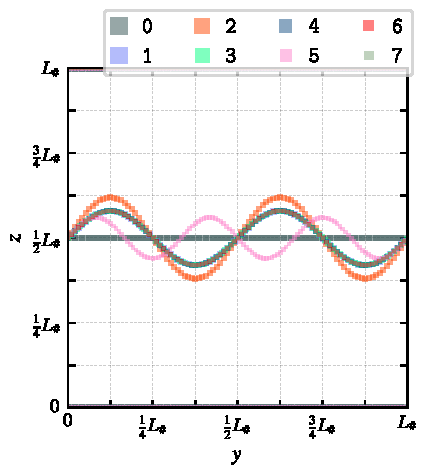
\includegraphics[width=0.4\textwidth]{../../figs/Methodology/initial_perturbations.pdf}
    % \end{figure}
    % }

% *************************************
% NOTES *******************************
\begin{notes}[3][sims]
    \itnote{1}{
        \item \textcolor{O1}{For reference, \dots}
        \item We account for the small difference in perturbation from PT to sim. onset.
        }
    \nnote{2}{Baseline/benchmark}
    \nnote{3}{Vary one parameter at a time}
\end{notes}
% *************************************

\end{frame}


\begin{uioimageframe}[info={}]{figs/initial_perturbations.pdf}
    {
    \newcommand{\INC}[1]{\(#1\mathcolor{uiogreen2}{\nearrow}\)}
    \newcommand{\DEC}[1]{\(#1\mathcolor{uiopink2}{\searrow}\)}
    \begin{table}
        {\small{\begin{tabular}{@{}cl@{}}
            % \pause
            \uncover<2>{\simO & \DEC{\epsast }} \\
            \simI & ---\\
            % \midrule
            \simII & \INC{\epsast}\\
            \simIII & \INC{N_\#}\\
            \simIV & \INC{L_\#} \\
            \simV & \INC{p} \,\,\, \DEC{\epsast} \,\,\, \INC{N_\#} \\
            \uncover<2>{\simVI & \DEC{\xi_\ast} }\\
            \simVII &  \DEC{(a\ped{i}-a_\ast)}
        \end{tabular}}}
    \end{table}}

% *************************************
% NOTES *******************************
\begin{notes}[2][initial perturbations]
    \nnote{1}{}
    \nnote{2}{{From here: Will ignore simulations 0 and 6.}}
\end{notes}
% *************************************
\end{uioimageframe}


% |||||||||||||||||||||||||
% |||||| DW dynamics ||||||
% |||||||||||||||||||||||||

% \subsection{Findings}
\subsection{DW}

% \begin{frame}{Time measures \comment{remove?}}
%     % Time variables
%     \begin{description}
%         \item[\descItem{scale factor} ] $\only<3>{\mathcolor{uioblue1}}{a}= \pclosed{1+\redshift}^{-1} = a_\ast s^\alpha$
%         \item[\descItem{cosmic redshift} ] $\redshift=1/a - 1$
%         \item[\descItem{conformal time} ] $s= \tau/\tau_\ast$
%         \item[\descItem{scale-dependent time parameter} ] $\only<3>{\mathcolor{uioblue1}}{t_\omega} \equiv \omega (s-1) = p(\tau-\tau_\ast)$
%         \item[\descItem{phase-transition time-scale} ] $\chi_+ \equiv \sqrt{1-\upsilon} = \sqrt{1-{(a_\ast/a)}^3}= \sqrt{1-s^{-3\alpha}}$ 
%     \end{description}
%     \uncover<2->{
%     \bigskip
%     Matter domination $\leftrightarrow$ $\alpha=2$}
% \end{frame}




\begin{frame}{Wall displacement field}
    Center wall's $z$-position $z\ped{w}=z_0 + \epsilon(\tau, x, y)$ where $z_0 = \mathfrak{D} \equiv L_\#/2$ is the unperturbed position and 
    \( \epsilon(\tau, x, y) = \varepsilon(\tau) \sin(py) \) the displacement field.
    \medskip

    \begin{description}[font=\scshape]
        \item[\descItem{first approach}]<2-> $\leadsto$ $\varepsilon(\tau) = \epsA(\tau)$, analytically determined in the thin-wall limit 
        \item[\descItem{second approach}]<3-> $\leadsto$ $\varepsilon(\tau) = \epsB(\tau)$, from the coordinate at which the simulated field $\abs{\chi}$ takes its minimum value along a slice at a $y$-coordinate that satisfies $\sin(py)=1$ %\note<3>{Intricate way of saying, see next slide}
    \end{description}
    
    \medskip
    \uncover<4>{We do \textcolor{R1}{not} expect a perfect match.}

% *************************************
% NOTES *******************************
\begin{notes}[4][DW]
    \nnote{1}{}
    \nnote{2}{One single solution when normalised and plotted over the time parameter $t_\omega=\omega(s-1)$}
    \nnote{3}{Intricate way of saying, see next slide}
    \itnote{4}{
        \item Initially defn. not thin, and very close to anti-wall.
        \item Spatial resolution might not capture sinus wave.
        \item \textbf{Inter- and intra-wall forces}
        \item Asymptotic field inhabits oscillations that might affect both wall thickness, but more importantly surface tension, and then again the eom for $\varepsilon$.
        \item \textcolor{O1}{To mention some\dots}
    }
\end{notes}
% *************************************

\end{frame}

\begin{frame}[plain]%{%
    % \centering
%     % \vspace*{-3mm}
    % ****** ANIMATION ******
    \ifCompAnims
        \animategraphics[loop,keepaspectratio,width=\columnwidth,height=\textheight,autoplay]{50}{gifs/eps_achi2/eps_achi2-}{0}{182}
    \else
        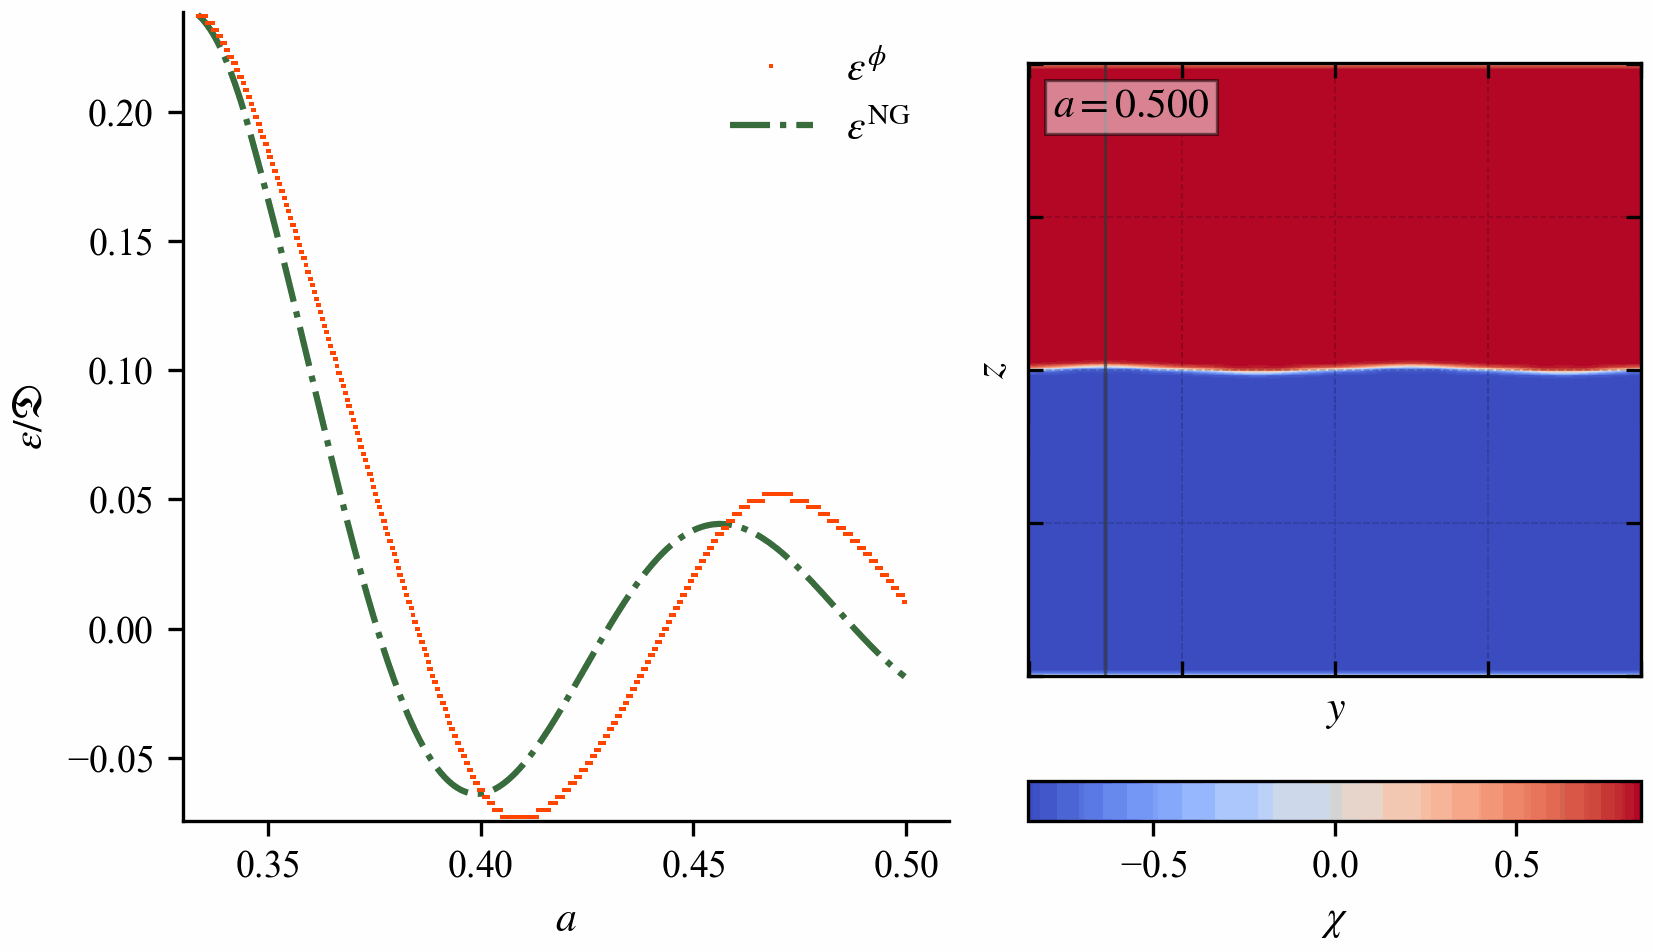
\includegraphics[keepaspectratio,width=\columnwidth,height=\textheight]{gifs/eps_achi2/eps_achi2-182}
    \fi
    % ***********************

% *************************************
% NOTES *******************************
\notesImage[{\textit{Simulation 2:} ``Worst one,'' but visually the clearest\par}
{Take the opportunity to point out a few weaknesses:}
{--Inter- and intra-wall forces}][animation (sim 2)]
% *************************************
\end{frame}

% \uiofullpageimage{gifs/eps_achi2/eps_achi2-182}

% \begin{frame}{idk}
\uiobigimage{Wall position $e=\varepsilon/\epsast$ as functions of $t_\omega=p(\tau-\tau_\ast)$}{../../figs/Findings/eps_diff_sims_combi.pdf}{$e\equiv\varepsilon/\epsast, \quad \Delta e \equiv \abs*{\epsA-\epsB}, \quad t_\omega = \omega (s-1)$}%
\notesImage[This x-axis is not time][combi plot]

% \uiofullpageimage{../../figs/Findings/eps_diff_sims_combi.pdf}
% \end{frame}















% |||||||||||||||||
% |||||| GWs ||||||
% |||||||||||||||||


\subsection{GWs}

\begin{frame}{Gravitational waves}
    % Only monochromatic plus-polarised waves are 
    \begin{textblock*}{\paperwidth-0.3cm}(0.0cm,0.3cm)
        \begin{flushright}
            \ifOnlyNotes\else
            \invisible<1>{\fcolorbox{B3}{B3}{\footnotesize\color{white}{
            \(a\tilde{h}_+^{\text{\tiny{NG}},\phi} \propto \integ{\hat{\tau}}\bclosed{\dots} \cross \Bessel[\ell] \big(\bclosed{\dots} p \varepsilon^{\text{\tiny{NG}},\phi}\big) \)
            }}}
            \fi
        \end{flushright}
    \end{textblock*}

    We have GWs in Fourier space with $\vec{k}=(k_x, k_y, k_z) = (\mathtt{u}, \mathtt{v}, \mathtt{w}) k_\#$. 

    \medskip

    \begin{description}[font=\scshape]
        \item[\descItem{\(\hpA \)}]<2-> $\leftrightarrow$ semi-analytical formula with $\epsA$ as input to the SE tensor
        \item[\descItem{\(\hpB \)}]<2-> $\leftrightarrow$ semi-analytical formula with $\epsB$ as input to the SE tensor
        \item[\descItem{\(\hpC\)}]<3-> $\leftrightarrow$ output from \asgrd
    \end{description}
    
    \bigskip
    \uncover<4->{\SideNote{Magnitudes.}{The magnitudes %$\tilde{h}^2 =\tilde{h}_+^\ast \tilde{h}_+$ 
    differ unsystematically inbetween these three, and we will not address this issue here.}}


    % \uncover<4->{Gravitational energy density:\citef[4]{maggioreGravitationalWavesVol2018}
    % \begin{equation}
    %     \rho\ped{gw} \simeq \frac{M\nped{Pl}^2}{2a^4} \avg{ \dot{\ah}^2_+ + \dot{\ah}^2_\times },
    % \end{equation}
    % where $\ah_P=ah_P$}

% *************************************
% NOTES *******************************
\begin{notes}[4]
    \itnote{1}{
        \item lack of summary statistic
        \item only FT of GWs
    }
    \nnote{4}{\textcolor{O1}{Only qualitative comparison.}}
\end{notes}
% *************************************
\end{frame}




\uiobigimage{Gravitational radiation \(  \rho\ped{gw} = M\nped{Pl}^2 a^{-2}\avg*{ \dot{h}\^{ij}\dot{h}\_{ij} } \)}{../../figs/Findings/avhijprimenorm.pdf}{\(s=\tau/\tau_\ast, \quad t_\omega= \omega(s-1) \)}\notesImage[\textcolor{G2}{SKIP?}][gravitational rad.]




% \begin{frame}{\unfinishedSlide~Limitations}

%     \begin{itemize}
%         \item<1-> Lack of summary statistic for $\hpAB$.
%         \begin{itemize}
%             \item Brute-force computation time-consuming and difference in magnitudes \comment{???}
%         \end{itemize}
%         \item<2-> Inverse Fourier transform is challeging to find analytically. 
%     \end{itemize}


%     \bigskip
%     % \uncover<3->{\paragraph{Peculiarity.}
%     % We have $\hpAB \in \Real$ in Fourier space for our setup, but simulated results suggest $\hpC = \hpCR + \im \, \hpCI\in \Complex$. Oddly enough, we find that $\hpCI\sim \hpB$ and $\hpCR \not\sim \hpB$.
%     % }


%     % \medskip
%     % Otherwise, we see that the difference $\Delta\varepsilon$ is significant in the computation of $h_+$.


%     % We have $\hpAB \in \Real$ in Fourier space for our setup. 
    
%     % Simulated results $\hpC = \hpCR + \im \, \hpCI\in \Complex$


%     % We find that $\hpCI\sim \hpB$

% % *************************************
% % NOTES *******************************
% \begin{notes}[2]
%     \nnote{1}{}
% \end{notes}
% % *************************************
% \end{frame}

\uiobigimage{}{../../figs/Findings/hp_kspace_sim1.pdf}{Sim.~\simnum{1}: \( \epsast=0.08_\#\), \( p= 2k_\#\)}
\notesImage[][peculiarity (sim 1)]


\uiobigimage{}{../../figs/Findings/hp_kspace_sim5.pdf}{Sim.~\simnum{5}: \( \epsast=0.06_\#\), \( p= 3k_\#\)}
\notesImage[][peculiarity (sim 5)]
% \note{\noteNext{We move on to a systematic summary of the presented results.}}




\subsection{Summary}


\begin{frame}[plain]%{Main results}
    % We use $e\equiv\varepsilon/\epsast$

    % \begin{minipage}{\textwidth}
    % \begin{table}
    % \begin{threeparttable}
    %     {
    %     \newcommand\YAY{\textcolor{G1}{yes}}
    %     \newcommand\NAY{\textcolor{R1}{no}}
    %     \newcommand\MAY{\textcolor{O1}{yes\tnote{*}}}
    %     % \renewcommand{\thefootnote}{\fnsymbol{footnote}}
    %     % -----------------------
    %     \begin{tabular}{@{}lcc@{}}
    %         & \tabHeading{Calculation} & \tabHeading{Simulation} \\
    %         \toprule
    %         % -----------
    %         \uncover<1->{$e$ independent of $\epsast$ & \YAY & \NAY } \\
    %         \uncover<2->{$e\not\sim s^{-5/2}\Cylindrical[-5/2](\omega s)$ & \YAY & \YAY} \\
    %         \uncover<3->{($e$ vs.~$t_\omega$)-plot indep. of parameters &\YAY & \MAY} \\
    %         % & \dots & \dots  \\
    %         \bottomrule
    %     \end{tabular}
    %     \uncover<3->{\begin{tablenotes}
    %         \item[*] To some extent.
    %     \end{tablenotes}}
    %     }
    % \end{threeparttable}
    % \end{table} 
    % \end{minipage}

    \begin{table}
    \begin{threeparttable}
        {
        \newcommand\YAY{\textcolor{G1}{yes}}
        \newcommand\NAY{\textcolor{R1}{no}}
        \newcommand\MAY{\textcolor{O1}{yes\tnote{*}}}
        % \renewcommand{\thefootnote}{\fnsymbol{footnote}}
        % -----------------------
        {\small{\begin{tabular}{@{}lcc@{}}
            & \tabHeading{Calculation} & \tabHeading{Simulation} \\
            \toprule
            % -----------   
            \tabSubheading{Wall position,} $e= \varepsilon/\epsast$ & $\epsA[e]$ & $\epsB[e]$\\
            \midrule
            % -----------
            \uncover<2->{$e$ independent of $\epsast$ & \YAY & \NAY } \\
            \uncover<3->{$e \sim s^{-5/2}\Cylindrical[-5/2](\omega s)$ & \NAY & \NAY} \\
            % \uncover<3->{$e\not\sim\zeta(s)$ & \YAY & \YAY} \\
            \uncover<4->{($e$ vs.~$t_\omega$)-plot indep. of parameters &\YAY & \MAY} \\
            \uncover<5->{$e$ unaffected by large fifth-force oscillations & \MAY & \MAY} \\
            % \uncover<5->{%
            \midrule
            \tabSubheading{Gravitational waves} & $\hpAB$ & $\hpC$ \\
            \midrule
            \uncover<6->{$\tilde{h}_\times=0$ &\YAY   & \YAY} \\
            \uncover<7->{$\tilde{h}_+\in \Real$ &\YAY   & \NAY} \\
            % \uncover<8->{$\tilde{h}_+\rvert_{k_x\neq 0} =0$ \& $\tilde{h}_+\rvert_{k_y\neq n p}=0 $ &\YAY   & \YAY} \\
            % \uncover<9->{$\tilde{h}_+\rvert_{k_z=0}=0 $ &\YAY   & \NAY} \\
            \uncover<8->{$\tilde{h}_+\simeq 0$ for $k_x\neq 0$, and for $k_y \neq np$ &\YAY   & \YAY} \\
            \uncover<9->{$\tilde{h}_+=0 $ for $k_y=0$ &\YAY   & \NAY} \\
            \bottomrule
        \end{tabular}}}
        \uncover<3->{\footnotesize{\begin{tablenotes} 
            \item[*] To some extent.
        \end{tablenotes}}}
        }
    \end{threeparttable}
    \end{table} 


% *************************************
% NOTES *******************************
\begin{notes}[9][summary (TABLE)]
    \nnote{1}{Summarise\dots}
    \nnote{3}{\textit{Is the time-dependence of the surface tension insignificant?}}
    \nnote{4}{\textit{Is there a single, common graph when normalised and plotted over $t_\omega$?}}
    \nnote{5}{Want to mention that the discrepancy does matter when computing the GWs, and that is why we insert this result into the formula for $h_+$}
\end{notes}
% *************************************

\end{frame}




